\documentclass[12pt,preprint]{aastex}

\usepackage{verbatim}
\usepackage{color}
\usepackage[normalem]{ulem} % for striking out with \sout
\usepackage{amsmath} % for boldsymbol
% A comment block

%\newcommand{\comment}[1]{}

% For color
\newcommand{\mpname}[1]{#1_color.eps}
\newcommand{\clraitoff}{red}
\newcommand{\lumblack}{(black)}
\newcommand{\lumblue}{(blue)}
\newcommand{\lumred}{(red)}
\newcommand{\vdisred}{(red-dashed curve)}
\newcommand{\vdisblue}{(blue-solid curve)}

% For bw
%\newcommand{\mpname}[1]{#1.eps}
%\newcommand{\clraitoff}{}
%\newcommand{\lumblack}{}
%\newcommand{\lumblue}{}
%\newcommand{\lumred}{}
%\newcommand{\vdisred}{(dashed curve)}
%\newcommand{\vdisblue}{(solid curve)}

\newcommand{\umag}{$u$}
\newcommand{\gmag}{$g$}
\newcommand{\rmag}{$r$}
\newcommand{\imag}{$i$}
\newcommand{\zmag}{$z$}
\newcommand{\gmr}{$g-r$}



\newcommand{\gammat}{$\gamma_T$}
\newcommand{\gammacross}{$\gamma_\times$}
\newcommand{\deltasig}{$\Delta \Sigma$}
\newcommand{\deltaplus}{$\Delta \Sigma_+$}
\newcommand{\deltacross}{$\Delta \Sigma_\times$}
\newcommand{\deltarho}{$\Delta \rho$}
\newcommand{\movr}{$M(<r)$}
\newcommand{\sigmacrit}{$\Sigma_{crit}$}

\newcommand{\photoz}{photo-z}
\newcommand{\photozs}{photo-zs}

\newcommand{\tlum}{$L^{tot}$}
\newcommand{\tngal}{$N_{gal}^{tot}$}

\newcommand{\lstarlim}{$0.4 L_*$}
\newcommand{\lvir}{$L_{200}$}
\newcommand{\nvir}{$N_{200}$}
\newcommand{\rvir}{$r_{200}^{gals}$}

\newcommand{\ngal}{$N_{gal}$}
\newcommand{\maxbcg}{maxBCG}
\newcommand{\numNgalBins}{12}
\newcommand{\numLumBins}{16}

\newcommand{\tngalAperture}{2$h^{-1}$ Mpc}

\newcommand{\photo}{\texttt{PHOTO}}
\newcommand{\astrop}{\texttt{ASTRO}}
\newcommand{\mt}{\texttt{MT}}
\newcommand{\spectro}{\texttt{SPECTRO}}
\newcommand{\spectroone}{\texttt{SPECTRO1d}}
\newcommand{\spectrotwo}{\texttt{SPECTRO2d}}
\newcommand{\target}{\texttt{TARGET}}

\newcommand{\lenszmax}{0.3}
\newcommand{\lenszmin}{0.05}

\newcommand{\photoversion}{\texttt{v5\_4}}

%\def\eone{e$_1$}
%\def\etwo{e$_2$}
\newcommand{\etan}{e$_+$}
\newcommand{\erad}{e$_\times$}
\newcommand{\eclass}{\texttt{ECLASS}}
\newcommand{\eclasscut}{-0.06}
\newcommand{\gmrcut}{0.7}

\newcommand{\hrs}{$^{\mathrm h}$}
\newcommand{\minutes}{$^{\mathrm m}$}

\newcommand{\ugriz}{$u, g, r, i, z$}
\newcommand{\polarization}{polarization}

\newcommand{\wgm}{$w_{gm}$}
\newcommand{\wgg}{$w_{gg}^p$}
\newcommand{\wmm}{$w_{mm}$}
\newcommand{\xigg}{$\xi_{gg}$}
\newcommand{\ximm}{$\xi_{mm}$}
\newcommand{\xigm}{$\xi_{gm}$}

\newcommand{\numspec}{127,001}
\newcommand{\numspecvlim}{10,277}
\newcommand{\numrand}{1,270,010}
\newcommand{\numspectot}{278,192}
\newcommand{\numvdis}{49,024}
%\newcommand{\numsource}{10,259,949}
% hirata: 
\newcommand{\nummask}{1,815,043}
\newcommand{\numTenMpc}{132,473}
\newcommand{\numThirtyMpc}{101,221}
\newcommand{\numsource}{27,912,891}

\newcommand{\numpairsTenMpc}{2,670,898,177}
\newcommand{\altnumpairsTenMpc}{2.7 billion}
\newcommand{\numpairsThirtyMpc}{14,818,082,122}
\newcommand{\altnumpairsThirtyMpc}{14.8 billion}



\newcommand{\xirmax}{$\xi_{gm}(R_{max})$}


\def\eps@scaling{1.0}% 

\newcommand{\sn}{$(S/N)$}
\newcommand{\Tsn}{$(S/N)_{\textrm{size}}$}
\newcommand{\fsn}{$(S/N)_{\textrm{flux}}$}

% stolen from the BA14 source
\newcommand{\vecg}{\mbox{\boldmath $g$}}
\newcommand{\vecD}{\mbox{\boldmath $D$}}
\newcommand{\vecQ}{\mbox{\boldmath $Q$}}
\newcommand{\matR}{\mbox{$\bf R$}}
\newcommand{\matC}{\mbox{$\bf C$}}
\newcommand{\bnabg}{ \boldsymbol{\nabla_g}}

\newcommand{\desreq}{$4\times 10^{-3}$}
\newcommand{\lsstreq}{$2\times 10^{-3}$}

\newcommand{\sersic}{S\'{e}rsic}

\slugcomment{Last revision \today}
\shortauthors{Sheldon}
\shorttitle{Bayesian Shear Estimation}

\begin{document}

\title{On Bayesian Shear Estimation}

\author{
Erin S. Sheldon\altaffilmark{1}
}

\altaffiltext{1}{Brookhaven National Laboratory, Bldg 510, Upton, New York 11973}


\begin{abstract}

    I present an implementation of the Bayesian shear estimation method of
    \cite{ba14}, in particular model-fitting approach.  In \cite{ba14}, the
    method was shown to be unbiased, but no implementation for fitting
    astronomical images was presented. I tested the implementation using
    simulated galaxy images modeled as \sersic\ profiles with $n=1/2, 1,
    \textrm{and} ~ 2$, and convolved with a PSF and flat pixel response
    function.  I used a simple Gaussian model for the PSF to avoid potential
    PSF-fitting errors, and I fit simulated images with the correct \sersic\
    model family to avoid model-bias.  I simulated galaxies with a discrete set
    of size ratios $\sigma_{gal}/\sigma_{PSF} = 1, 1.4, 2$ and a broad range of
    signal-to-noise ratios $S/N \in [10,1000]$. A constant shear was applied to
    all images.  In all cases I recover the input shear to better than 2 parts
    in a thousand, finding the largest error for the smallest galaxies. I
    suspect the remaining bias is due to details of the likelihood sampling
    technique, and can be improved upon.  This accuracy is sufficient for
    current and planned surveys.  

\end{abstract}

\section{Introduction} \label{sec:intro}

intro

\section{Algorithm} \label{sec:algo}

The full algorithm is presented in \citet[][BA14]{ba14}.  There are a few basic
assumptions underlying this approach.  Following the notation in BA14:

\begin{itemize}

    \item The shear is weak, $g \ll 1$.

    \item In the limit of weak shear, only the ensemble mean shear can be
        derived from galaxy shapes.

    \item The posterior distribution of the shear derived from a large ensemble
        of galaxy images is Gaussian.


\end{itemize}

The first assumption is true under most circumstances, but will break down
along lines-of-sight near large over-densities, such as clusters of galaxies.

The second assumption follows from the first, and the fact that galaxy images
are to be used to estimate the shear: galaxies have intrinsic shapes, with
variance larger than the typical shear induced by structures in our universe.
Given this limitation, the estimation of shears from individual sources is
abandoned.  This limitation would not apply if a large set of intrinsically
round, extended sources were found.

The third point follows from the central limit theorem: if the shear is derived
from a large enough ensemble of galaxy shapes, the posterior necessarily
approaches a Gaussian.

Under these assumptions, a second-order estimator was derived for the shear,
consistent with the assumption of a Gaussian posterior.  This form is a Taylor
expansion of the logarithm of the posterior for the shear, with shear as the
expansion variable:
\begin{equation} \label{eq:pexpand}
-\ln P(\vecg | \vecD) \approx {(\rm const)} - \ln P(\vecg) - \vecg \cdot \sum_i
    \frac{\vecQ_i}{P_i}
    + \frac{1}{2} \vecg \cdot \left[ \sum_i \left(\frac{\vecQ_i \vecQ^T_i}{P_i^2}
    - \frac{\matR_i}{P_i}\right) \right] \cdot \vecg,
\end{equation}
where \vecD\ is the data vector and \vecg\ is the two-component shear.  The
terms $P_i$, $\vecQ_i$, and $\matR_i$ are 
\begin{eqnarray} \label{eq:pqrdef}
P_i     & = & P(\vecD_i | \vecg=0) \nonumber \\
\vecQ_i & = & \left. \bnabg P(\vecD_i | \vecg)\right|_{\vecg=0} \\
\matR_i & = & \left. \bnabg \bnabg P(\vecD_i | \vecg)\right|_{\vecg=0}. \nonumber
\end{eqnarray}
$P$ is the bayesian ``prior'', and corresponds to the true distribution
of all the relevant galaxy parameters.

Prior information is key to this approach: these equations involve derivatives
of the un-lensed distribution of shapes, which is part of the prior $P$. To
predict the observed distribution of shapes in general, the un-lensed
distribution of shapes must be mathematically sheared and compared to
observables.  However in the approximation given above, only derivatives near
$g=0$ are required and the mean shear can be solved for:
\begin{eqnarray} \label{eq:shdef}
\matC_g^{-1} & = & \sum_i \left(\frac{\vecQ_i \vecQ^T_i}{P_i^2} - \frac{\matR_i}{P_i}\right) \\
\bar{\vecg} & = &  \matC_g \sum_i \frac{\vecQ_i}{P_i}.
\end{eqnarray}

In practice the shape of each galaxy is not precisely known. Instead, the
derivatives in equation \ref{eq:pqrdef} are marginalized over the full
likelihood distribution for each galaxy, and these marginalized values are used
in the aggregate shown in equation \ref{eq:shdef}.  

An approach to measuring non-constant shear is also given, as are third-order
tweaks to the second-order perturbations, but implementations of those ideas
are left to future work.

A full implementation, fitting to pixelized galaxy images, was not attempted in
\citet{ba14}.  The basic formalism was shown to work by generating shapes from
an analytic distribution, adding noise and shear, and recovering the underlying
shear using the second-order formula.

\section{Implementation} \label{sec:impl}

For this work a full implementation of the \citet{ba14} formalism was developed
to analyze noisy galaxy images smeared by a point spread function and 
pixelization.

As described in \S \ref{sec:algo}, the estimator involves integrals over the
full likelihood distribution for each galaxy.  Exploration of the likelihood
surface requires a large number of model evaluations.  As an optimization,
galaxy models were approximated as sums of Gaussians according the to the fits
in \citet{HoggGMix12}.  The PSF was also approximated using Gaussians.  This
use of Gaussians for both galaxy and PSF models facilitates analytic
convolutions of the galaxy model with the PSF.  This is a faster and simpler
alternative to convolutions using Fourier transforms. The use of the
Gaussian approximation introduces negligible bias in the recovered shear for
the sersic models fit in this work.

A fast, third order approximation to the exponential function was used for
rendering the galaxy and PSF profiles.  Even so evaluation of the exponential
function is the bottleneck for this calculation.

A Markov Chain Monte Carlo (MCMC) was used to explore the posterior surface.
Galaxies can have a wide variety of model parameters and errors in the best-fit
parameters.  It is not straightforward to predict what the parameter errors
will be before doing the full fit, making it difficult to choose a ``step
size'' for the MCMC chain.  For this reason an affine invariant MCMC method was
used, as first presented in \citet{GoodmanWeare10}.  The affine invariant MCMC
automatically adapts to the underlying distribution, so does not require tuning
the step size.  The python implementation presented in \citet{Mackey13} was
chosen for this work, as the rest of the algorithm and simulation were also
implemented in python.  For each galaxy, 80 ``walkers'' were used in the chain,
with 400 burnin steps and 200 steps per walker used for calculations.  This
number of steps may be excessive in some situations, but we found that accurate
results were obtained for the full range of parameters used in our simulations,
so we did not explore this further.

\section{A Note on Parametrization}

Because Gaussians were used for modeling both Galaxies and PSF, it is
convenient to parameterize objects in terms of the second moments rather than
alternative quantities such as half-life radii.  This parametrization is also
intuitive: for real images it is the unweighted second moments that are
modified by convolution with the PSF of instrument and atmosphere; the
covariance matrices simply add. Another way to put this is that it is the area
that is modified by the isotropic part of the PSF, and it is the ratio of areas
that controls the influence of the PSF on the shape of a galaxy.  The quantity
$T = I_{xx} + I_{yy}$, was chosen as a convenient size parameter, where
$I_{ij}$ is the unweighted second moment $\langle x_i x_j \rangle$.
The corresponding scale length can be written as $\sigma = \sqrt{T/2}$.

\section{Simulation} \label{sec:sim}

Pairs of galaxy images were generated at 90 degree offset in position angle, to
cancel shape noise.  This simulation strategy is known as a ``ring
test''\citep{Nakajima2007}, and greatly reduces the number of simulated images
required to test the shear code.

Two types of elliptical galaxy models were generated, exponential disks,
$\textrm{exp}(-r)$, and \devauc\ profiles, $\textrm{exp}(-r^{1/4})$.

Models were convolved with a simulated PSF, a single round Gaussian with
$\sigma = \sqrt{2}$ pixels $(T=4)$.  A simple PSF was chosen so that PSF
modeling was not a source of error in the shear recovery.  The models were also
convolved with square pixels of uniform response.

The un-lensed shape distribution was chosen to be identical to the toy
distribution used in \cite{ba14}.  This distribution is not a good description
of real galaxy shapes, but was chosen for consistency with that work.  That
distribution also has the required property that it is twice differentiable.

The other galaxy parameters were drawn from simple distributions.  The size
parameter $T=I_{xx} + I_{yy}$ was drawn from a log-normal distribution with
scatter of 15\%.  The total flux was drawn from a log-normal with 30\% scatter.
The centroid was drawn from a Gaussian in each coordinate, with $\sigma$ of 0.2
pixels.

Four suites of simulations were run:  Two runs with exponential disks and two
with \devauc\ profiles.  For each galaxy type, two different galaxy sizes were
chosen: $\sigma_{g}/\sigma_{\textrm{PSF}} = \{1.4,2.0\}$, which corresponds to
$T_{g}/T_{\textrm{PSF}} =\{2,4\}$.


\section{Fitting Simulated Galaxies} \label{sec:simfit}

The simulated images were fit using parametrized models as presented in \S
\ref{sec:impl}.   A Gaussian was fit to a rendered, pixelized PSF model, and
the full, convolved model was generated by analytically convolving the galaxy
model with this PSF model. By using a fit to the observed, pixelized PSF, the
convolution by the pixels is built in to the PSF model. Thus the analytic
convolution of PSF with galaxy model accounts for the all PSF and pixel
effects.  

While a single Gaussian does perfectly model a {\it pixelized} Gaussian PSF, in
practice the single Gaussian is sufficient for the resolution of these
simulations ($\sigma_{\textrm{PSF}}=\sqrt{2}$).  For a less well sample PSF, a
more complex model would be required.

Prior distributions were chosen to match exactly the true distributions used in
the simulation.  The correct model was fit in each case; i.e. when simulating
exponential disks, an exponential disk was fit.  By choosing the true priors
and model, the accuracy of the algorithm is tested without confusion with other
issues such as model bias or empirical prior determination.

\section{Results} \label{sec:results}

\subsection{Calibration Bias vs. \sn} \label{sec:snbias}

Figure \ref{fig:fracerr} contains results for each of the four simulation
suites discussed in \S \ref{sec:sim}, representing different galaxy types and
sizes. 

\begin{figure}[p] \centering
 \centering 
 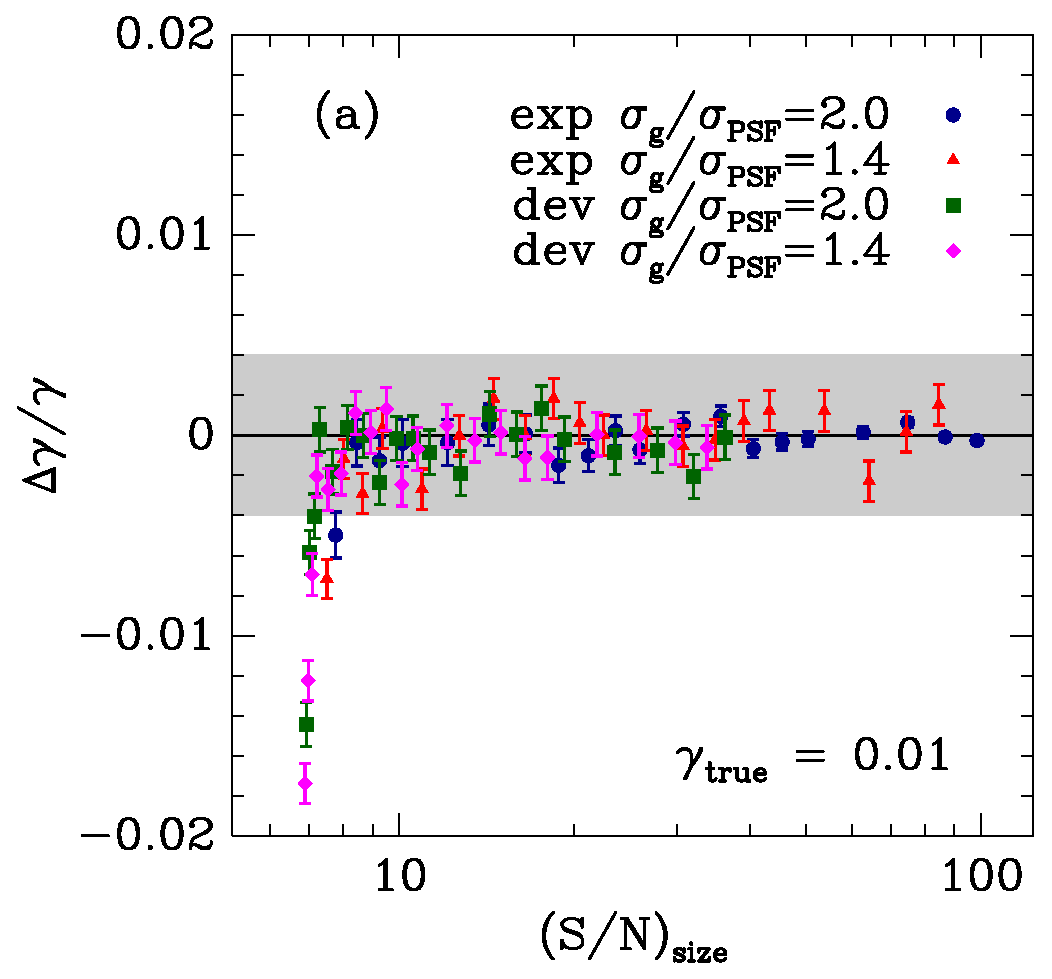
\includegraphics[scale=0.45]{figures/cbafit-geg-T-s2n.eps}
 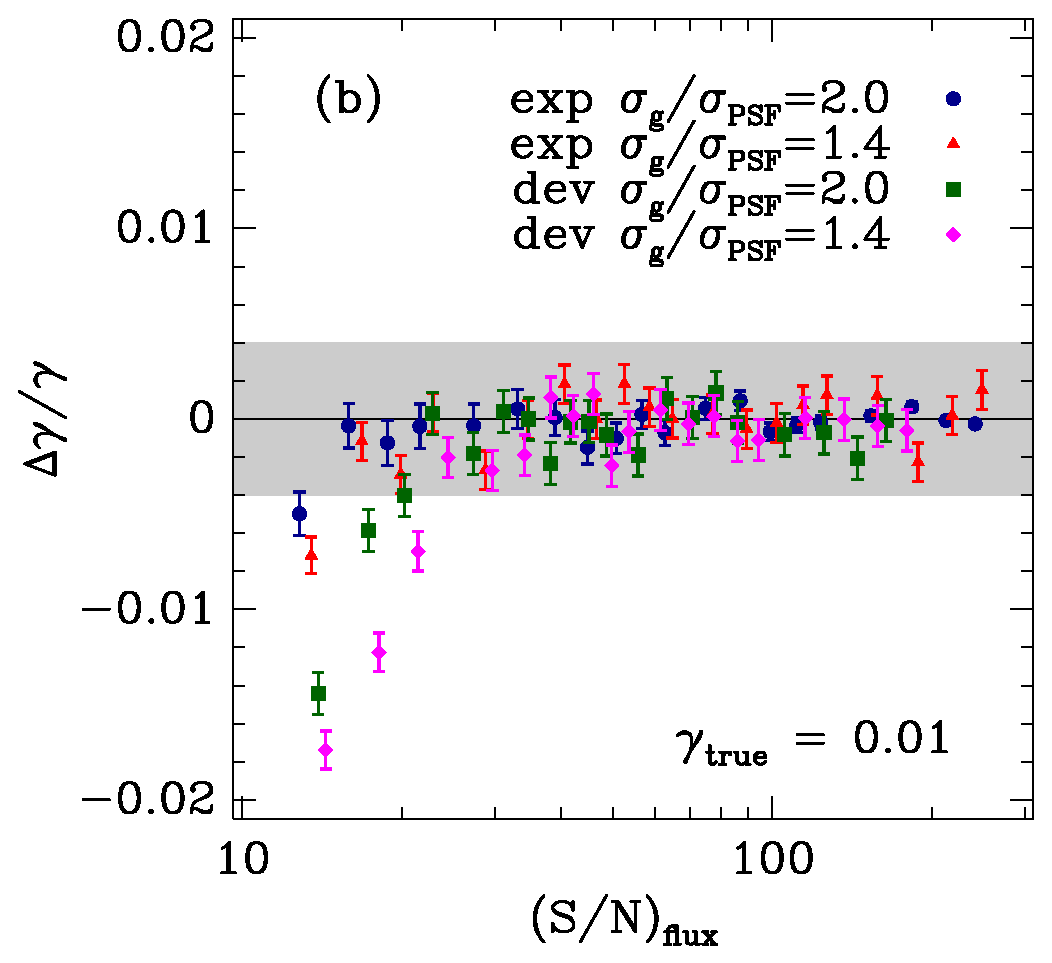
\includegraphics[scale=0.45]{figures/cbafit-geg-flux-s2n.eps}

 \caption{ Fractional bias in the recovered shear for the estimator presented
     in \cite{ba14}.  The bias is plotted as a
     function of galaxy signal-to-noise ratio $(S/N)$, for various galaxy
     properties and two different measures of $(S/N)$.  In panel (a) is
     plotted \Tsn, where the measure of intrinsic galaxy size is $T=I_{xx} + I_{yy}$.  In 
     panel (b) is plotted \fsn.  The flux and $T$ are parameters in the model
     fits, and the associated $(S/N)$ is the ratio of best-fit value to error in
     the fit.  In each panel the fractional error is plotted for galaxies of
     different size and type, as described in the text.  As shown panel (a)
     panel, the bias depends uniquely on \Tsn\ for different galaxy types and
     sizes.  However, \fsn\ is not a sufficient descriminator for different
     galaxy types and sizes.  The \Tsn\ can be used to remove galaxies from the
     sample that will yield poor shear estimates, independent of galaxy
     properties, but not so \fsn.  For \Tsn$~ \gtrsim 10$ this shear estimator meets
 the accuracy requirements for the Dark Energy Survey, shown as the gray band.
 \label{fig:fracerr}}

\end{figure}

The fractional bias is shown as a function of signal-to-noise ratio $(S/N)$,
for two definitions of $(S/N)$, \Tsn\ and \fsn.  The traditional measure of
signal-to-noise ratio is \fsn, defined as the best fit value of total flux
divided by the error in the fit.  A more useful definition of signal-to-noise
ratio is \Tsn, the signal-to-noise ratio of the galaxy intrinsic, pre-seeing
size.  As expected, fits to noisy galaxies will result in a noisy determination
of size, and also a noisy shear measurement. But small galaxies are also more
difficult to fit, even at higher values of flux signal-to-noise ratio.  Thus it
is intuitive that small galaxies may also yield poor shear estimates.

The fractional bias in the recovered shear is, within errors, uniquely
determined by \Tsn.  But for \fsn, the fractional bias depends also on galaxy
type and size, indicating the \fsn\ is not a sufficient statistic for
determining the bias.

\subsection{Calibration Bias vs. True Shear} \label{sec:truebias}

Figure \ref{fig:nonoise} contains results for a zero-noise simulation.  The
fraction bias is shown as a function of true shear.  The bias follows deviates
from zero as a quadratic function of the true shear.  The red curve shows a
best-fit quadratic function, and is fully consistent with the data.  This
quadratic error expected, since the formulas for the ensemble shear are expanded
to second order.

\begin{figure}[t] \centering
 \centering 
 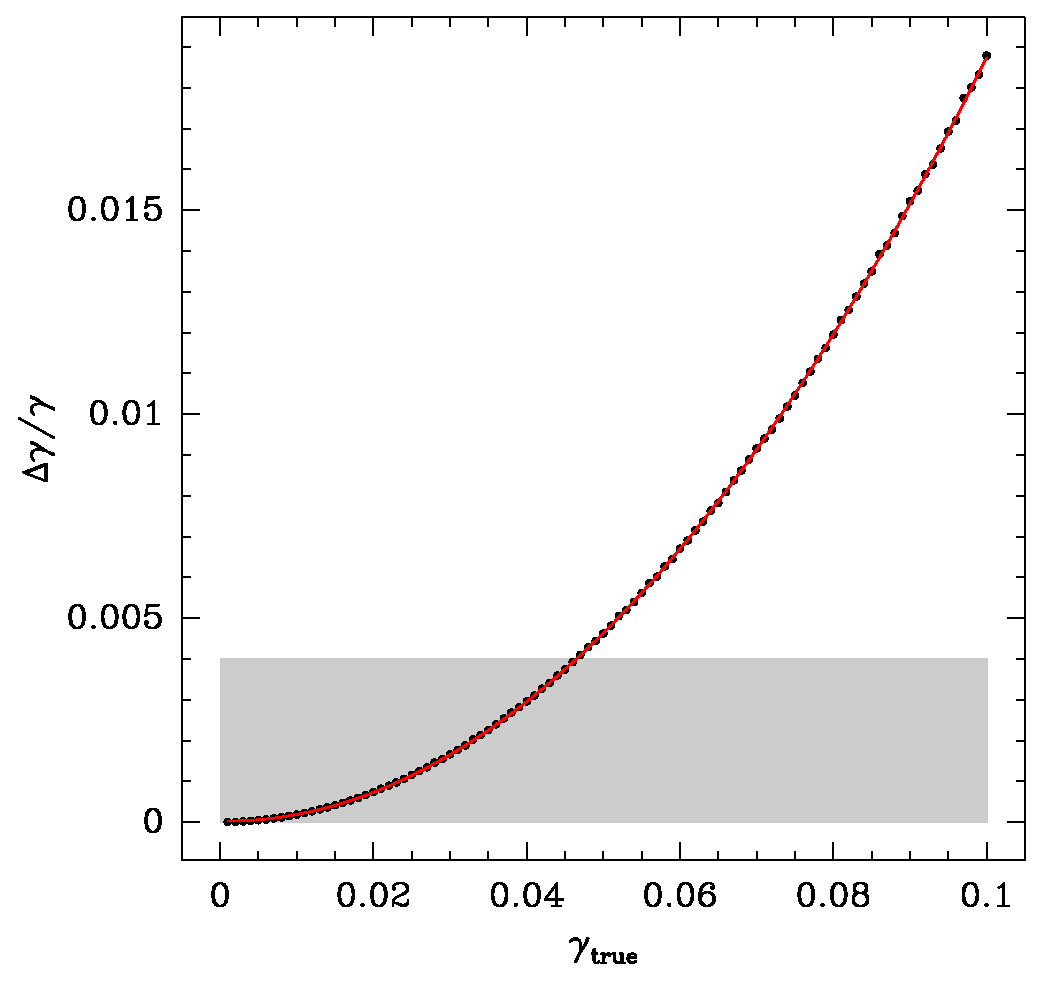
\includegraphics[scale=0.6]{figures/fracerr-vs-shear.eps}

 \caption{Fractional bias in the recovered shear as a function of true shear,
     in a zero noise simulation.  The solid curve is the best-fit quadratic
     function of the true shear.  The quadratic bias as a function of true
     shear indicates a break down of the second-order approximation presented
     in \cite{ba14}. The gray band represents the requirements for the Dark
 Energy Survey. \label{fig:nonoise}}

\end{figure}

\subsection{Comparison to Dark Energy Survey Requirements} \label{sec:desreq}

Figure \ref{fig:fracerr} contains a gray band representing the requirements for
shear recovery in the Dark Energy Survey \citep[][DES]{DESWhitePaper}.  The
method meets DES survey requirements when using galaxies that have intrinsic
sizes measured with \Tsn$ \gtrsim 10$.  Note no unique value of the traditional
flux signal-to-noise ratio \fsn\ is sufficient to choose such galaxies.  More
simulation statistics are needed to study the requirements for future surveys
with tighter calibration requirements.

Figure \ref{fig:nonoise} also contains a gray band representing DES
requirements.  For shears greater than about 0.05, the Taylor expansion
approximation is no longer sufficient to meet DES requirements.  An
implementation to higher order, a different expansion, or perhaps a full
mapping of the posterior of the shear will be required to recover larger shears
to sufficient accuracy.

\section{Summary} \label{sec:summary}

The Bayesian shear estimator presented in \cite{ba14} can be used to accurately
recover gravitational shear in a galaxy population, as long as the underlying
true distribution of all galaxy parameters is known and the sizes of the
individual galaxies can be precisely determined.  For example, if the
signal-to-noise ratio of the size \Tsn\ is greater than $\sim$10, the shear
can be determined to $\Delta g/g \sim10^{-3}$, sufficient for current surveys such as DES.

A generic conclusion of this study is that the signal-to-noise ratio of the
estimated intrinsic galaxy size, \Tsn, is a good indicator of how well the
shear can be recovered.  This was also found for other estimators, such as that
presented in \cite{Miller07}, although that result is not shown in this work.
The traditional signal-to-noise ratio \fsn\ was not found to correlate well
with shear accuracy across different galaxy types and sizes.

The estimator used in this work, an approximate expansion of the posterior of
the shear to second order, was shown to break down at higher shears. This is as
expected.  For shears greater than about 0.05, the systematic error introduced
is larger than the baseline requirements of current experiments such as DES.
In order to accurately measure larger shears, an alternative approximation or a
full mapping of the shear posterior is required.

A model fitting approach was used in this work, but true galaxies cannot be
fully described by a finite number of parameters.  \cite{Kacprzak13} show that
this ``model bias'' may be on the order of baseline requirements for surveys
such as DES, and potentially crippling for future surveys with more stringent
requirements. One potential solution is to fit models with more freedom, and
appropriately choose galaxies with well measured sizes.  \cite{ba14} propose an
alternative to the model-fitting technique based on moments in Fourier space
which makes no explicit parameterization of galaxy light distributions.  An
evaluation of this model free approach in the presence of noise will be the
subject future work.

\section*{Acknowledgments}

ES is supported by DOE grant DE-AC02-98CH10886.

Thanks to Gary Bernstein, Bob Armstrong, and Anze Slosar for many useful
discussions.  Thanks to the STAR and LBNE experiments at BNL for use of spare
cycles on their compute clusters, and to the RACF staff at BNL for support.


\bibliographystyle{apj}
% Bib database
\bibliography{apj-jour,astroref}

\end{document}

